%%%%%%%%%%%%%%%%%%%%%%%%%%%%%%%%%%%%%%%%%
% University Assignment Title Page 
% LaTeX Template
% Version 1.0 (27/12/12)
%
% This template has been downloaded from:
% http://www.LaTeXTemplates.com
%
% Original author:
% WikiBooks (http://en.wikibooks.org/wiki/LaTeX/Title_Creation)
%
% License:
% CC BY-NC-SA 3.0 (http://creativecommons.org/licenses/by-nc-sa/3.0/)
% 
% Instructions for using this template:
% This title page is capable of being compiled as is. This is not useful for 
% including it in another document. To do this, you have two options: 
%
% 1) Copy/paste everything between \begin{document} and \end{document} 
% starting at \begin{titlepage} and paste this into another LaTeX file where you 
% want your title page.
% OR
% 2) Remove everything outside the \begin{titlepage} and \end{titlepage} and 
% move this file to the same directory as the LaTeX file you wish to add it to. 
% Then add \input{./title_page_1.tex} to your LaTeX file where you want your
% title page.
%
%%%%%%%%%%%%%%%%%%%%%%%%%%%%%%%%%%%%%%%%%
%\title{Title page with logo}
%----------------------------------------------------------------------------------------
%	PACKAGES AND OTHER DOCUMENT CONFIGURATIONS
%----------------------------------------------------------------------------------------

\documentclass[12pt]{article}
\usepackage{wrapfig}
\usepackage[english]{babel}
\usepackage[utf8]{inputenc}
\usepackage{amsmath}
\usepackage{graphicx}
\usepackage[colorinlistoftodos]{todonotes}

\begin{document}

\begin{titlepage}

\newcommand{\HRule}{\rule{\linewidth}{0.5mm}} % Defines a new command for the horizontal lines, change thickness here

\center % Center everything on the page
 
%----------------------------------------------------------------------------------------
%	HEADING SECTIONS
%----------------------------------------------------------------------------------------

\textsc{\LARGE Universidad de Sonora}\\[1.5cm] % Name of your university/college
\textsc{\Large Física Computacional I}\\[0.5cm] % Major heading such as course name
%\textsc{\large Evaluación }\\[0.5cm] % Minor heading such as course title

%----------------------------------------------------------------------------------------
%	TITLE SECTION
%----------------------------------------------------------------------------------------

\HRule \\[0.4cm]
{ \huge \bfseries Evaluación 1}\\[0.4cm] % Title of your document
\HRule \\[1.5cm]
 
%----------------------------------------------------------------------------------------
%	AUTHOR SECTION
%----------------------------------------------------------------------------------------

\begin{minipage}{0.4\textwidth}
\begin{flushleft} \large
\emph{Autor:}\\
Manuel I. \textsc{Gómez G.} % Your name
\end{flushleft}
\end{minipage}
~
\begin{minipage}{0.4\textwidth}
\begin{flushright} \large
\emph{Profesor:} \\
Carlos \textsc{Lizárraga Celaya} % Supervisor's Name
\end{flushright}
\end{minipage}\\[2cm]

% If you don't want a supervisor, uncomment the two lines below and remove the section above
%\Large \emph{Author:}\\
%John \textsc{Smith}\\[3cm] % Your name

%----------------------------------------------------------------------------------------
%	DATE SECTION
%----------------------------------------------------------------------------------------

{\large 9 de marzo del 2018}\\[1cm] % Date, change the \today to a set date if you want to be precise

%----------------------------------------------------------------------------------------
%	LOGO SECTION
%----------------------------------------------------------------------------------------


\includegraphics[width=5.5cm]{Logo.jpg}\\[1cm] % Include a department/university logo - this will require the graphicx package
 
%----------------------------------------------------------------------------------------

\vfill % Fill the rest of the page with whitespace

\end{titlepage}

\section{Introducción}
El presente reporte evidencia todos los pasos que se siguieron a fin de concretar la primer evaluación semestral. A lo largo del presente documento se mostraran los resultados al manejar los datos (gráficas) y se contestarán ciertas preguntas con el fin de interpretar dichos resultados.

\section{Descripción de la estructura de los datos}
Los archivos que contenían todos los datos utilizados fueron $sargento\_201117.csv$ y $sargento\_salinidad\_201117.csv$. Ambos con diversas columnas que registraban mediciones del nivel del mar, temperatura del agua, presión, salinidad, conductancia y la fecha con hora de registro para cada uno de los datos.

En un principio existia una diferencia en la cantidad de datos entre ambos archivos, pero fue solucionada al momento de leer los archivos, comenzando la lectura desde otro punto y posteriormente eliminamos la columna que nos es innecesaria en ambos archivos.

\begin{figure}[h!]
\centering
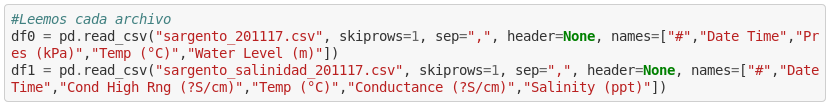
\includegraphics[height=2cm]{Lectura}
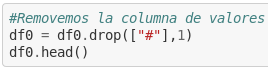
\includegraphics[height=2cm]{Columna}
\end{figure}

Ahora verificamos los datos capturados en el archivo con la función mostrada en la imagen anterior \textbf{df0.head()} para \textbf{sargento\_201117.csv} y \textbf{df1.head()} para \textbf{sargento\_salinidad\_201117.csv}.

\textbf{1)} Datos de sargento\_201117.csv
\begin{figure}[h!]
\centering
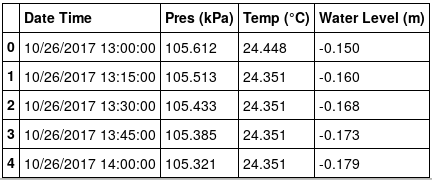
\includegraphics[width=6.5cm]{Tabla1}
\end{figure}

\textbf{2)} Datos de sargento\_salinidad\_201117.csv
\begin{figure}[h!]
\centering
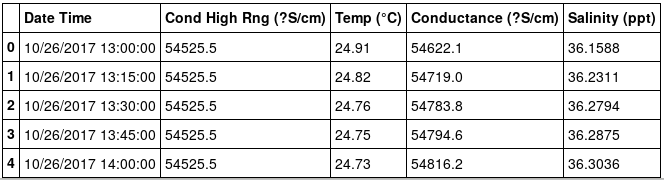
\includegraphics[height=3cm]{Tabla2}
\end{figure}


\section{Gráficas de caja}
Haciendo uso la biblioteca \textbf{Seaborn} se nos pide que generemos tres distintas gráficas de caja. Antes de poder hacerlo debemos transformar la fecha (\textbf{Date Time}) que fue capturada como un objeto en una variable de tiempo (\textbf{Ndate} y \textbf{month}).

Se aplica el código tanto para \textbf{df0} como \textbf{df1}.

\begin{figure}[h!]
\centering
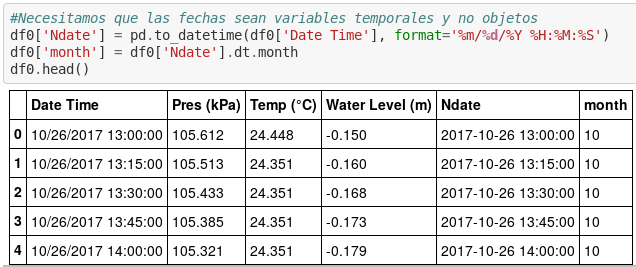
\includegraphics[width=10cm]{FechaVariable}
\end{figure}

Ahora que tenemos una variable de tiempo aplicamos los siguientes códigos, según el caso:
\\ \textbf{I.} Nivel del Mar (metros).
\begin{center}
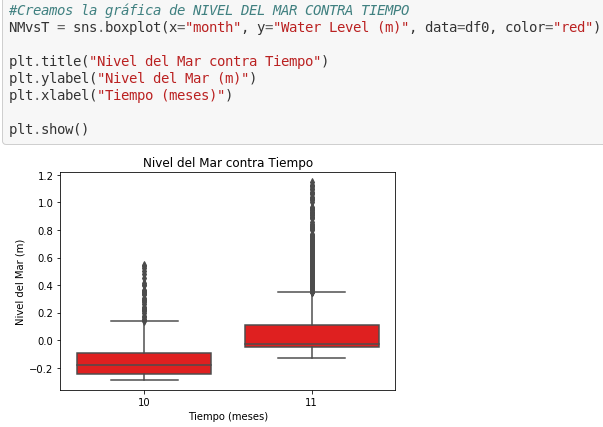
\includegraphics[height=8cm]{GrafCaja1}
\end{center}


\noindent \textbf{II.} Salinidad (Partes por mil - ppm).\\
\begin{figure}[h!]
\centering
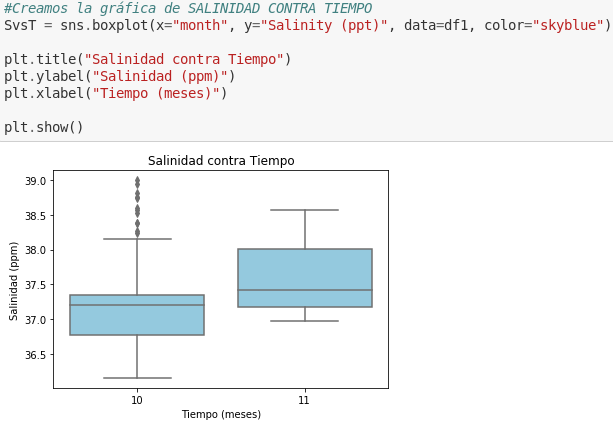
\includegraphics[height=8cm]{GrafCaja2}
\end{figure}

\textbf{ III.} Temperatura del Agua ($^{\circ}$C).
\begin{figure}[h]
\centering
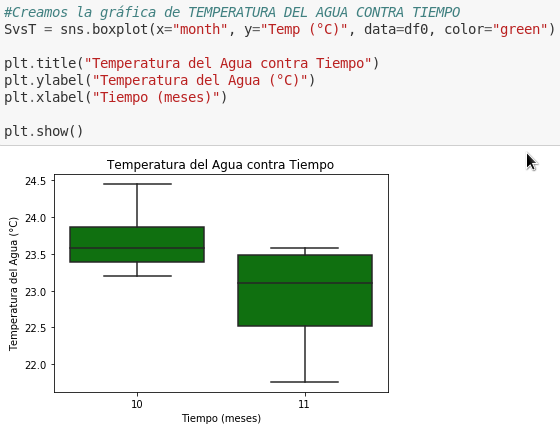
\includegraphics[height=8cm]{GrafCaja3}
\end{figure}

De igual forma es posible verificar o conocer específicamente los datos del gráfico si usamos la función \textbf{describe}, ya que al correr dicho código se nos genera una tabla que cuenta con los datos estadísticos generales para cada una de las columnas.

\begin{figure}[h]
\centering
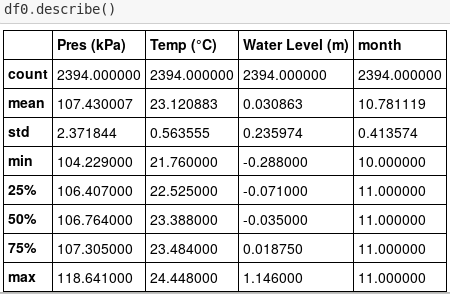
\includegraphics[height=6cm]{Describe1}
\end{figure}

\begin{figure}[h]
\centering
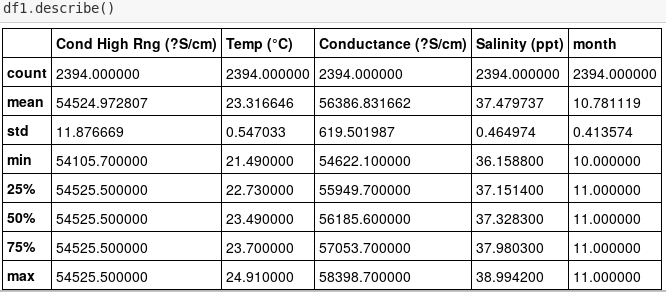
\includegraphics[width=14cm]{Describe2}
\end{figure}


\section{Regresión lineal: correlación entre variables}
Para llevar a cabo la regresión lineal y verificar si existe dicha correlación
es necesario tener todos los datos en un sólo DataFrame, por lo que debemos de unificar \textbf{df0} y \textbf{df1} para crear \textbf{df2}.

Primero, eliminemos las columnas $Date$ $Time$, $Temp$ $(^{\circ}C)$, $Ndate$ y $month$ de \textbf{df1} debido a que son columnas ya existentes en \textbf{df0}. \\ \\

\vfill

\begin{figure}[h]
\centering
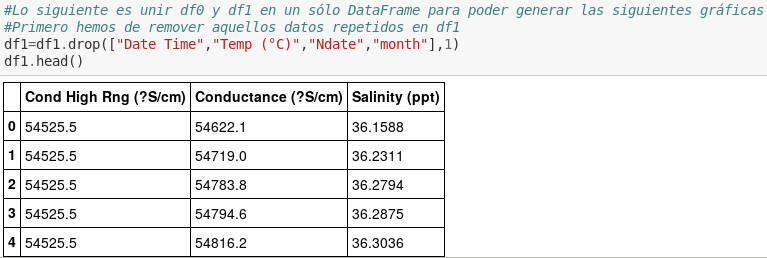
\includegraphics[height=4.5cm]{ElimColum}
\end{figure}

Ahora que las columnas repetidas han sido eliminadas es más sencillo unir los DataFrames. El código utilizado es el siguiente:
\\

\begin{figure}
\centering
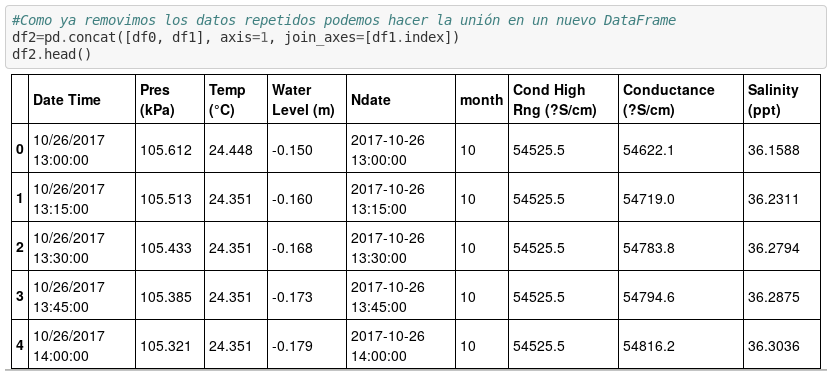
\includegraphics[width=15cm]{Unir}
\end{figure} 

Tras haber hecho eso, podemos proseguir a realizar la regresión lineal usando \textbf{Seaborn}. Para generarlas usaremos los siguientes código:\\
\textbf{I.} Nivel del Mar - Salinidad.

\begin{figure}[h!]
\centering
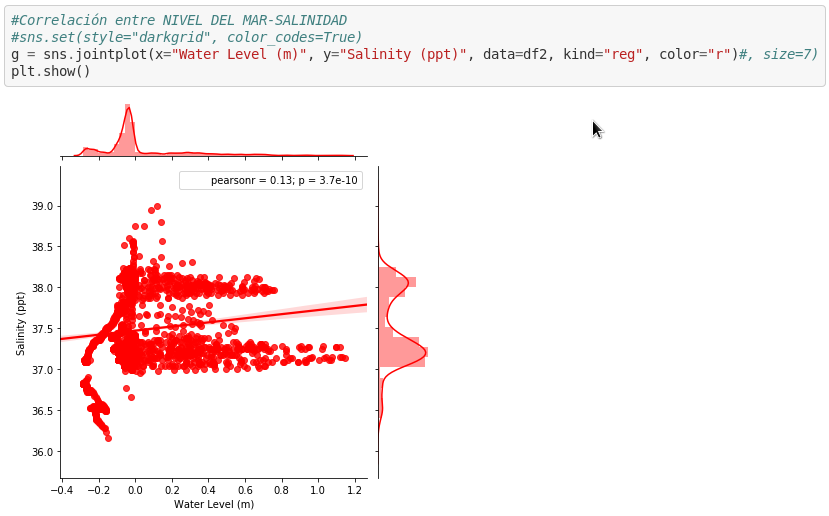
\includegraphics[height=7cm]{GrafCorre1}
\end{figure}

\noindent \textbf{II.} Nivel de Mar - Temperatura del Agua\\
\begin{center}%[h!]
%\centering
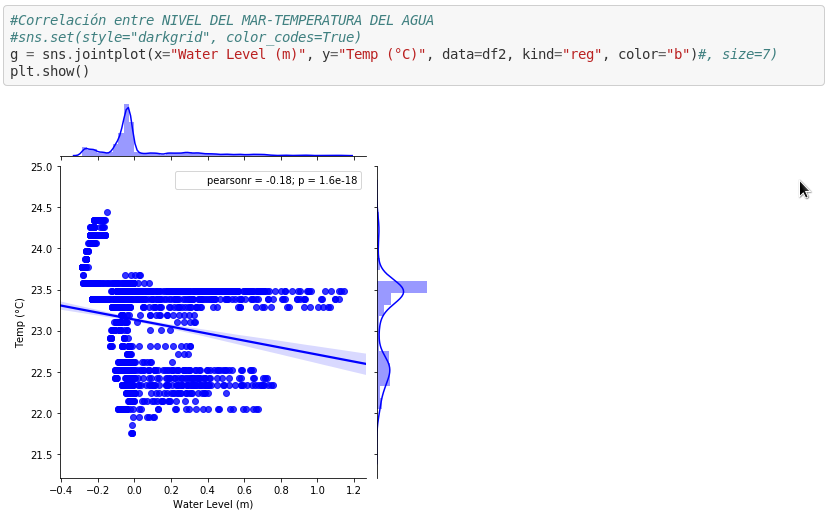
\includegraphics[height=8cm]{GrafCorre2}
\end{center}

\vfill

\noindent \textbf{ III.} Salinidad - Temperatura del Agua.\\
\begin{figure}[h]
\centering
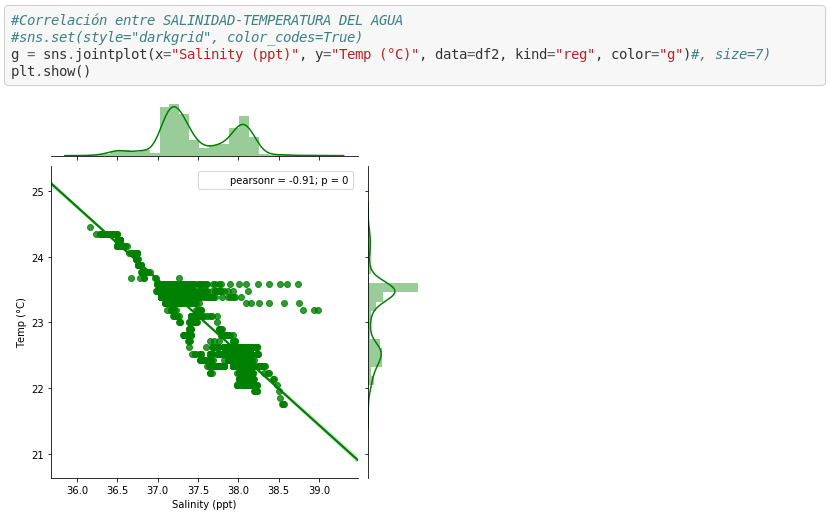
\includegraphics[height=8cm]{GrafCorre3}
\end{figure}

Al observar las gráficas vemos los distintos comportamientos que tiene una variable con respecto a la otra y en base a ello determinamos que no existe una correlación entre Nivel del Mar-Salinidad y Nivel del Mar-Temperatura del Agua, sin embargo, la última de ellas muestra que efectivamente entre la salinidad y la temperatura del agua se aprecia dicha correlación.

\section{Gráficas contra el tiempo}
En este punto se nos pide generar gráficas para cada una de las variables con las que hemos estado trabajando (Nivel del Mar, Temperatura del Agua y Salinidad) en función del tiempo.

Esta sección de la actividad es muy parecida pues sólo basta con cambiar los nombres de las variables para generar las distintas gráficas.\\
\\ \textbf{I.} Nivel del Mar en función del Tiempo

\begin{center}
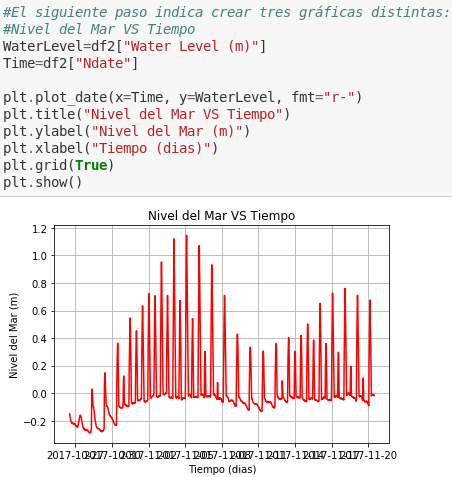
\includegraphics[height=11cm]{GrafT1}
\end{center}


\textbf{II.} Salinidad en función del Tiempo
\begin{center}
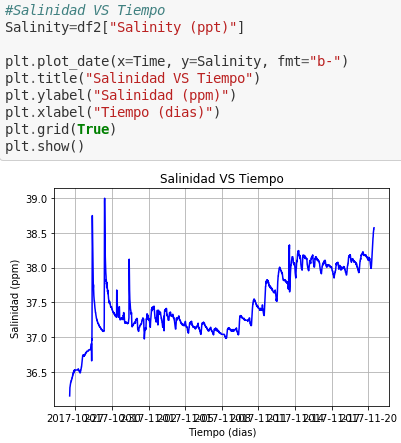
\includegraphics[height=8.5cm]{GrafT2}
\end{center}


\textbf{III.} Temperatura del Agua en función del Tiempo
\begin{center}
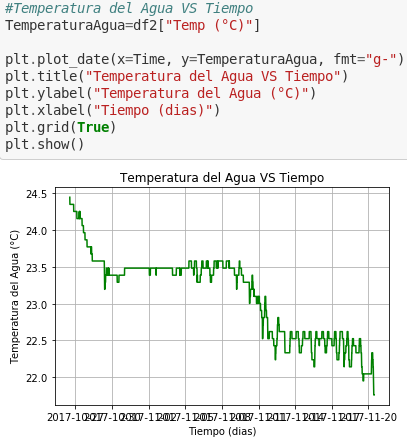
\includegraphics[height=8.5cm]{GrafT3}
\end{center}

%\begin{table}
%\centering
%\begin{tabular}{l|r}
%Item & Quantity \\\hline
%Widgets & 42 \\
%Gadgets & 13
%\end{tabular}
%\caption{\label{tab:widgets}An example table.}
%\end{table}

\section{Gráficas de doble eje}
Este tipo de gráficas ahora implican sobreponer los datos de dos de nuestras variables permitiendonos observarlas en el eje $y$ a lo largo del mismo intervalo de tiempo.

La diferencia aquí sería el establecer que es una gráfica de doble eje. En el siguiente código se muestra cómo se hizo.\\

\noindent \textbf{I.} Nivel del Mar y Salinidad
\begin{center}
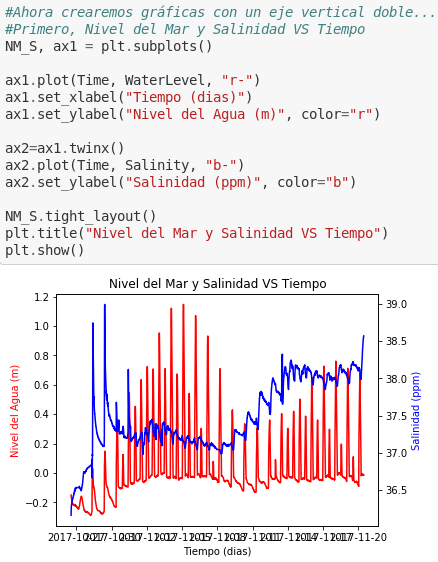
\includegraphics[height=10cm]{GrafDob1}
\end{center}

\textbf{II.} Nivel del Mar y Temperatura
\begin{center}
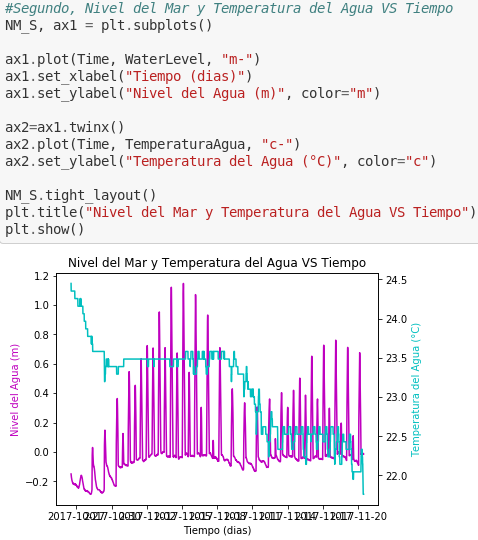
\includegraphics[height=8.5cm]{GrafDob2}
\end{center}


\section{Estableciendo límites}
Por último, debemos de crear nuevamente las gráficas de eje doble con la pequeña modificación de que ahora delimitaremos el eje del tiempo a solamente 5 días de la muestra total, de este modo podremos ver más a detalle el comportamiento para posteriormente dar nuestra conclusión acerca de las gráficas.
\\ El código empleado para esta actividad fue el siguiente:

\noindent \textbf{I.} Nivel del Mar y Salinidad
\begin{center}
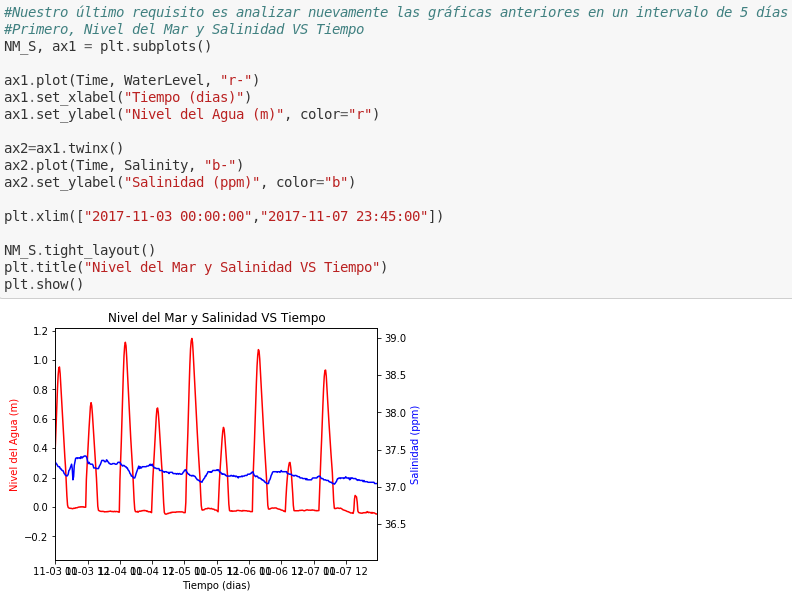
\includegraphics[height=9cm]{GrafDias1}
\end{center}

\textbf{II.} Nivel del Mar y Temperatura
\begin{center}
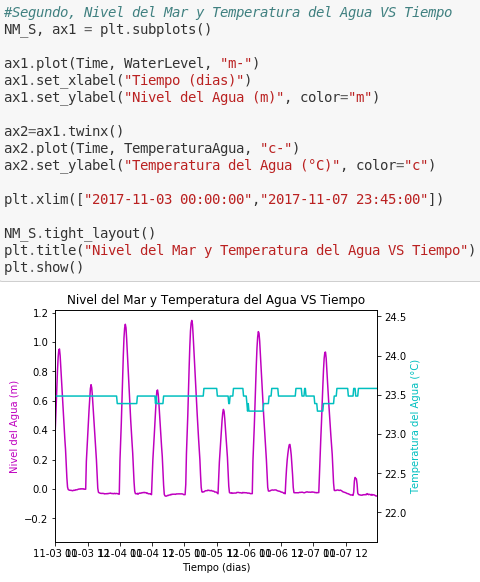
\includegraphics[height=9cm]{GrafDias2}
\end{center}

Ahora que podemos apreciar más detalladamente las gráficas hemos de notar la relación existente entre las variables.

A partir del gráfico del Nivel del Mar y Salinidad en función del Tiempo podríamos decir que en el momento en que aumenta el Nivel del Mar, lo cual implica que aumenta la marea, la salinidad se reduce, esto podría ser por la forma en que se ve distribuida en presencia de agua dulce.

La gráfica del Nivel del Mar y Temperatura del Agua en función del Tiempo muestra que a la llegada de agua dulce con el aumento de la marea la temperatura desciende unas cuantas décimas de grado centígrado, en cuanto no llegue nuevamente agua está aumenta de igual forma una pequeña fracción de grado.

\end{document}